\section{Results and Analysis}
We chose to prove our PoC using two scenes from Bitterli's 32 resources \cite{resources16}: \textit{The Wooden Staircase} and \textit{Utah Teapot}. These two were chosen for providing a collection of varied directives.

\textit{The Wooden Staircase} makes use of image-based textures, area lighting and has a vast array of different kinds of materials, including bumpmaps. The scene has a whopping set of 774 3D meshes - which makes it very difficult to convert manually.

\textit{Utah Teapot} is a much simpler scene, with one material and one 3D mesh. However, it uses a primitive checkerboard texture and environment mapping.

The scenes were rendered using Mitsuba 0.5.0, PBRT v3 and LuxRender v1.6 on a UNIX system running Ubuntu 14.04 LTS.

We rendered the original scenes for Mitsuba, PBRT and LuxRender and then the scenes converted from these input files by our system. The original scenes for Mitsuba and PBRT were the ones provided by Bitterli, while the LuxRender scenes were generated using the converter.

\begin{figure}[h]
\centering
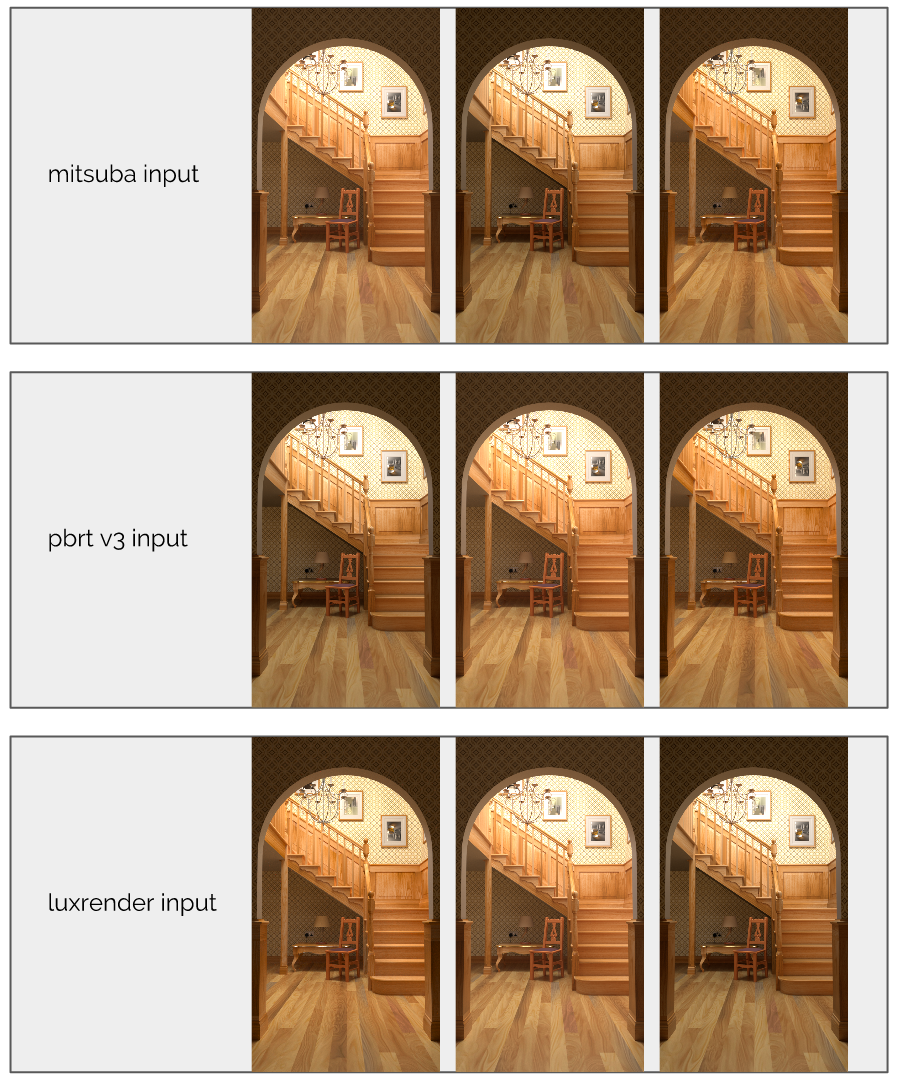
\includegraphics[width=5in]{figs/4_results/results_staircase.png}
\caption{Results for \textit{The Wooden Staircase} with Mitsuba, PBRT v3 and LuxRender input files.}
\label{fig:staircase}
\end{figure}

\begin{figure}[h]
\centering
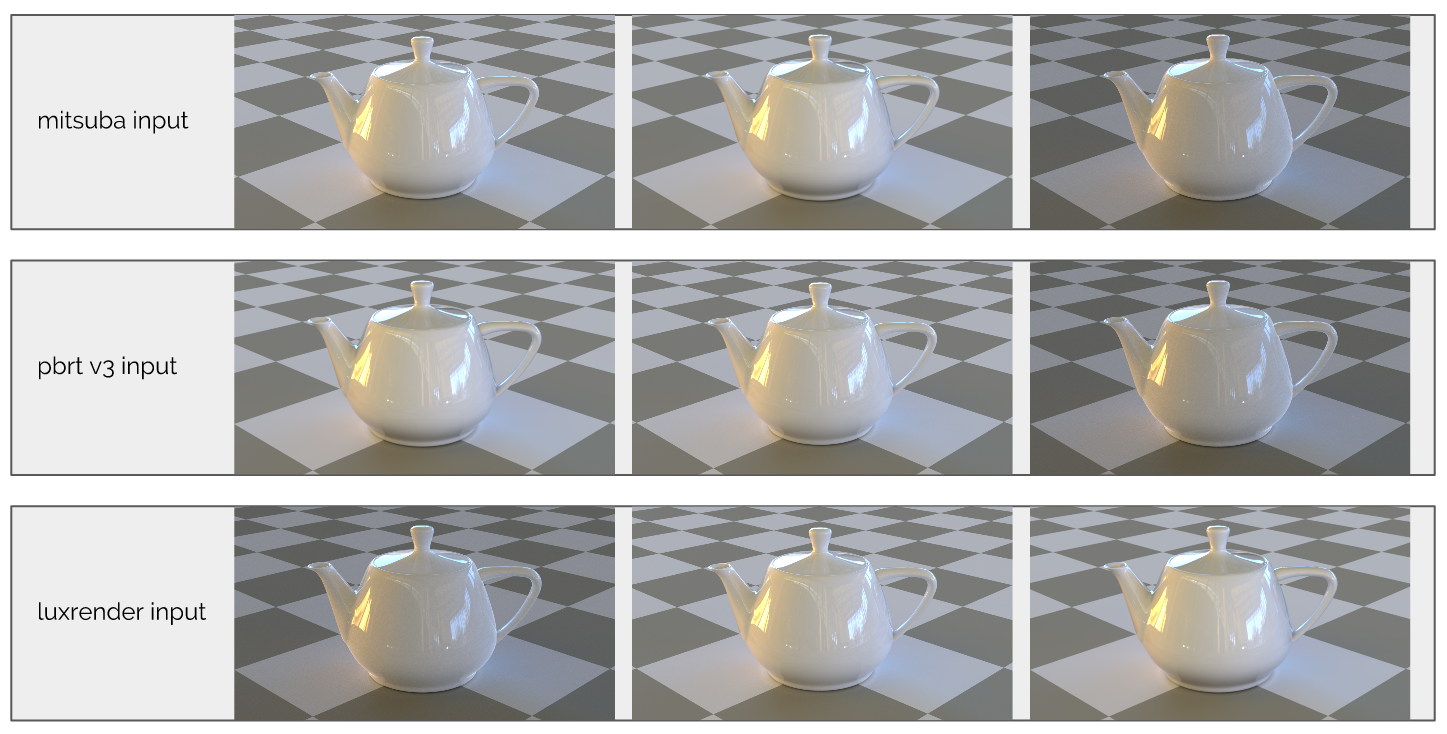
\includegraphics[width=5in]{figs/4_results/results_teapot.png}
\caption{Results for \textit{Utah Teapot} with Mitsuba, PBRT v3 and LuxRender input files.}
\label{fig:teapot}
\end{figure}

Insert commentary here.

\subsection{Limitations}
We decided to restrict the number of directives interpreted and converted in order to quickly produce a valid PoC.

In general, directives present in only one renderer were not added to the system, such as Mitsuba-only materials like \textit{phong} or \textit{blendbsdf}.

Our converter cannot interpret participating media or volumes. It also cannot convert mask materials and textures. For LuxRender, our converter cannot color metal materials given the issues discussed in \ref{systemarch}.
